\section{Arrivée en Inde}

31 janv. 2008

\begin{multicols}{2}

Bonjour tout le monde,

Ca y est nous voila arrivés, le vol s'est très bien passé, et l'arrivée à l'aéroport était assez mouvementée... même à 1h du matin vous n'imaginez pas le monde qu'il peut y avoir dans l'aéroport de Delhi.

\hspace*{-0.65cm}
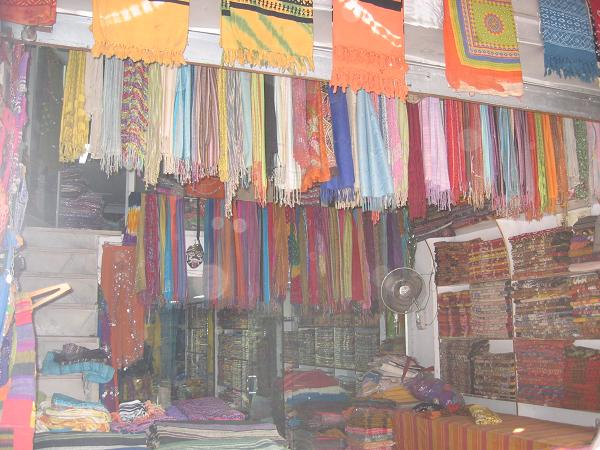
\includegraphics[width=4.8cm]{articles/Arrivee-en-inde/magasin.jpg}

Premier passage obligé par arnaques et compagnie, il ne faut même pas faire confiance à la banque de l'Inde pour le change... résultat 400 roupies dans le vent (bon ok, pour nous c'est pas grand chose 1 euro = 56 roupies).

\hspace*{-0.65cm}

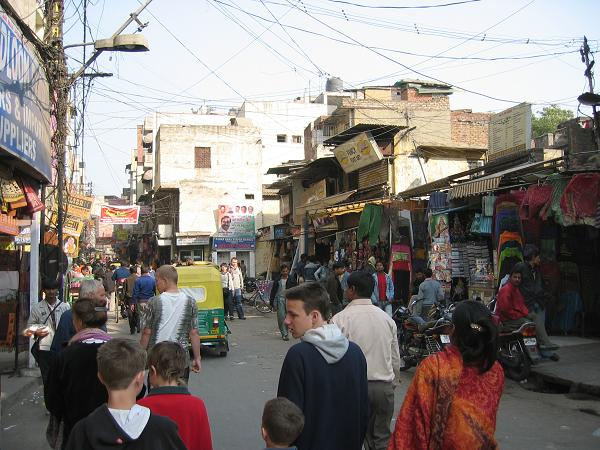
\includegraphics[width=4.8cm]{articles/Arrivee-en-inde/rue.jpg}

Puis nous avons déjoué les arnaques du chauffeur de taxi qui nous emmène vers une office du tourisme à 2h du mat déjà c'est louche, alors quand on voit qu'il ne fait pas le bon numéro et qu'il a un petit sourire aux lèvres, plus confiance. Au final c'est nous qui avons guidé notre chauffeur qui faisait exprès de se perdre (et qui au final nous demande de repayer la course alors que c'était un taxi prépayé).

Au final nous voila dans un petit hôtel tout minable du vieux Delhi, en plein milieu de Main Bazar, mais qu'est-ce qu'on est heureux...

A bientôt.


\end{multicols}

\bigskip
\textbf{\textsc{Commentaires}}

\medskip
Titou a écrit le 31 janv. 2008 :
\begin{displayquote}
YEAH !!!!
Content de vous savoir arrivés ! Moi je dis vive la mise en ligne des articles via les USA :D Amusez-vous bien et profitez de vos vacances bande de veinards ! A ploutch
\end{displayquote}

\medskip
Peggy a écrit le 31 janv. 2008 :
\begin{displayquote}
Ah bah non, on commençait à s'habituer aux posts réguliers nous\dots Bon, vivement quelques photos!
\end{displayquote}

\medskip
Nath a écrit le 31 janv. 2008 :
\begin{displayquote}
Et bien voilà vous y voilà  et l'aventure commence
Bon courage, profitez bien\dots de ces vacances méritées. Félicitations d'ailleurs.
A bientot.
\end{displayquote}

\medskip
Catherine a écrit le 1 fév. 2008 :
\begin{displayquote}
C'est sûr, ça ne vaudra jamais les photos que nos deux voyageurs nous montreront, mais à cette adresse, on peut avoir une petite idée des beautés que vous découvrirez en direct: http://www.linternaute.com/voyager/asie/inde-du-nord-le-royaume-des-maharadjas/inde-du-nord-le-royaume-des-maharadjas.shtml
Bien sûr, ce message s'adresse plus à ceux qui sont derrière leur ordi plutôt qu'à Cécile et Etienne\dots Bisous à vous deux
\end{displayquote}

\medskip
Gerien a écrit le 4 fév. 2008 :
\begin{displayquote}
Héhé,
Cécile, Etienne ?Z'êtes sûr de pas être ailleurs qu'en Inde ?
Parce que l'hôtel, les tapis de partout et la foule, ça ressemble comme qui dirait au Maroc :)
\end{displayquote}

\medskip
Tatid a écrit le 21 fév. 2008 :
\begin{displayquote}
Sympa les arnaques\dots Ralala les gens qui profitent des touristes, c'est quand même pas vachement sympa quoi\dots !
En tous cas, vous avez l'air + qu'heureux, bon séjour à vous deux !
\end{displayquote}

\vfill

